\hypertarget{rotationMatrix_8cpp}{\section{rotation\-Matrix.\-cpp \-File \-Reference}
\label{d9/d5c/rotationMatrix_8cpp}\index{rotation\-Matrix.\-cpp@{rotation\-Matrix.\-cpp}}
}


\-Definition of the \hyperlink{classRotationMatrix}{\-Rotation\-Matrix} class member functions.  


{\ttfamily \#include \char`\"{}rotation\-Matrix.\-h\char`\"{}}\*
\-Include dependency graph for rotation\-Matrix.\-cpp\-:
\nopagebreak
\begin{figure}[H]
\begin{center}
\leavevmode
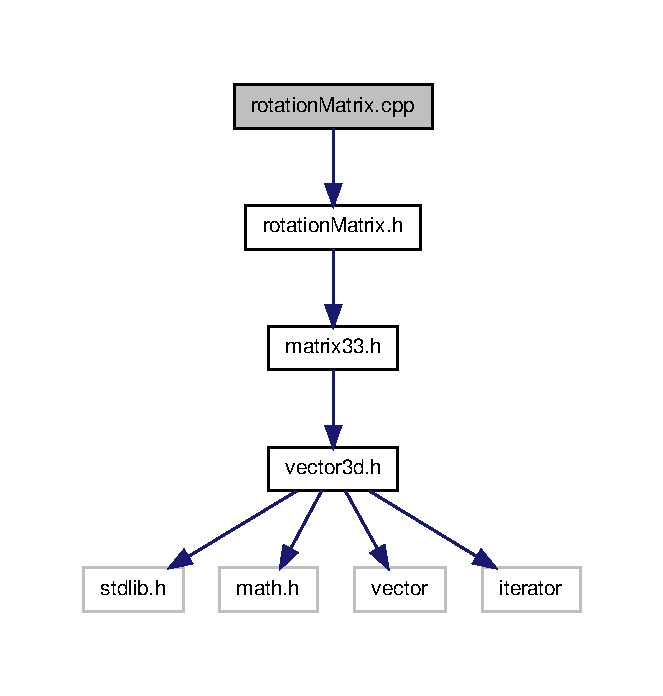
\includegraphics[width=318pt]{d8/d52/rotationMatrix_8cpp__incl}
\end{center}
\end{figure}


\subsection{\-Detailed \-Description}
\-Definition of the \hyperlink{classRotationMatrix}{\-Rotation\-Matrix} class member functions. \begin{DoxyAuthor}{\-Author}
\-Adhish \-Majumdar 
\end{DoxyAuthor}
\begin{DoxyVersion}{\-Version}
0.\-0 
\end{DoxyVersion}
\begin{DoxyDate}{\-Date}
25/04/2013
\end{DoxyDate}
\-This file defines member functions of the \hyperlink{classRotationMatrix}{\-Rotation\-Matrix} class for carrying out 3\-D rotations and axes transformations. 

\-Definition in file \hyperlink{rotationMatrix_8cpp_source}{rotation\-Matrix.\-cpp}.

